%File: formatting-instruction.tex
\documentclass[letterpaper]{article}
\usepackage{aaai}
\usepackage{times}
\usepackage{helvet}
\usepackage{courier}
\frenchspacing
% some very useful LaTeX packages include:
\usepackage{graphicx}  
\usepackage{amsmath}   
%\usepackage{fancyhdr}
%\usepackage{citesort}
%\usepackage{comment}

\setlength{\pdfpagewidth}{8.5in}
\setlength{\pdfpageheight}{11in}
\pdfinfo{
/Title (Modeling Human Workload in Unmanned Aerial Systems)
/Author (J. J. Moore, R. Ivie, T.J. Gledhill, E. Mercer and M. A. Goodrich)}
\setcounter{secnumdepth}{0}  
 \begin{document}
% The file aaai.sty is the style file for AAAI Press 
% proceedings, working notes, and technical reports.
%
\title{Modeling Human Workload in Unmanned Aerial Systems}
\author{J. J. Moore, R. Ivie, T.J. Gledhill, E. Mercer and M. A. Goodrich\\
Computer Science Department \\ Brigham Young University \\ Provo, UT\\
}
\maketitle
\begin{abstract}
%\begin{quote}
Unmanned aerial systems (UASs) often require multiple human operators fulfilling diverse roles for safe correct operation.  Although some persuasively dispute the utility of minimizing the number of humans needed to administer a UAS~\cite{MurphyBurke2010}, it is a long-standing objective for many designers.  This paper presents work toward understanding how workload is distributed between multiple human operators and multiple autonomous system elements in a UAS across time, with an ultimate goal to reduce the number of humans in the system. The approach formally models the {\em actors} in a UAS as a set of communicating finite state machines, modified to include a simple form of external memory. The interactions among actors are then modeled as a directed graph.  The individual machines, one for each actor in the UAS, and the directed graph are augmented with workload metrics derived from a review of the relevant literature. The model is implemented as a Java program, which is analyzed by the Java Pathfinder (JPF) model checker. JPF generates workload profiles showing how workload changes through time.  To demonstrate the utility of the approach, this paper presents a case study on a wilderness search and rescue (WiSAR) UAS analyzing two different mission outcomes. The generated workload profiles are shown to be consistent with known features of actual workload events in the WiSAR system. 
%\end{quote}
\end{abstract}

\noindent \section{Introduction}

Unmanned aerial systems (UASs), ranging from large military-style Predators to small civilian-use hovercraft, usually require more than one human to operate.  It is perhaps ironic that a so-called ``unmanned'' system requires multiple human operators, but when a UAS is part of a mission that requires more than moving from point A to point B, there are many different tasks that rely on human input including: operating the UAS, managing a payload (i.e., camera), managing mission objectives.  Some persuasively argue that this is desirable because different aspects of a mission are handled by humans trained for those aspects~\cite{MurphyBurke2010}. Human resources are expensive, and many others argue that it is desirable to reduce the number of humans involved.

However, the question of {\em how} to reduce the number of humans while maintaining a high level of robustness is an open question.  Some progress has been made by improving autonomy using, for example, automatic path-planning~\cite{WongBourgaultFurukawa2005,878915,pettersson2006probabilistic,QuigleyBarberEtAl2005,NelsonBarberMcLainBeard2006}, and automated target recognition~\cite{MorseEnghGoodrich2010,dasgupta2008multiagent,barber2006vision}.  However, careful human factors suggest that the impact of changes in autonomy are often subtle and difficult to predict, and this decreases confidence that the combined human-machine system will be robust across a wide range of mission parameters~\cite{KaberEndsley2004,chen2011supervisory,chen2007human}.

We argue that one reason for the limitations of prior work in measuring workload is that the level of resolution is too low.  For example, although the NASA TLX dimensions include various contributing factors to workload (e.g., physical effort and mental effort), the temporal distribution of workload tends to be ``chunked" across a period of time.  Secondary task measures can provide a more detailed albeit indirect breakdown of available cognitive resources as a function of time~\cite{kaber1999adaptive}, but with insufficient explanatory power for what in the task causes workload peaks and abatement.  Cognitive workload measures, including those that derive from Wickens' multiple resource theory~\cite{wickens2002multiple}, provide useful information about the causes of workload spikes, but these measures have not been widely adopted; one way to interpret this paper is as a step toward robust implementations of elements of these measures.  Finally, measures derived from cognitive models such as ACT-R are providing more low-level descriptions of workload which potentially include a temporal history~\cite{lebiere2013cognitive}, but these approaches may require a modeling effort that is too time-consuming to be practical for some systems.

This paper presents a model of four human roles for a UAS-enabled wilderness search and rescue (WiSAR) task, and is based on prior work on designing systems through field work and cognitive task analyses~\cite{Adams2008,GoodrichMorse2008}.  We first identify a suite of possible workload measures based on a review of the literature.  We then consider seven {\em actors} in the team: the UAV, the operator and the operator's GUI, the video analyst and the analyst's GUI, the mission manager, and a role we call the ``parent search'' which serves to connect the UAS technical search team to the other components of the search enterprise.  We present the formal model of each of these actors using finite state machines, and then discuss how the connections between these state machines defines what we call a {\em Directed Team Graph} (DiTG) that describes who communicates with whom and under what conditions.  We then augment the model to be able to encode specific metrics based on a subset of the measures identified in the literature.  Using the Java PathFinder model checker, we then create temporal profiles for each of the workload metrics and check consistency of the temporal profiles by associating workload peaks and abatements with likely causes. 


\section{Workload Categories}

In this section, we present a brief review of the set of workload categories from which we distill a set of workload metrics.  We restrict attention to three general categories of workload metrics: cognitive, temporal, and algorithmic.  A fourth relevant workload category is the cost of maintaining team constructs like shared situation awareness~\cite{EliasFiore2011}, but we leave a discussion of team-related workload to future work.



\subsection{Cognitive}
Cognitive workload describes the difficulties associated with managing various signals, decisions, and actions relevant to a particular task or goal~\cite{MorayEtAl91,lebiere2013cognitive,Goodrich2004,Chadwick2004}. We adopt a simple form of Wickens' multiple resource theory~\cite{wickens2002multiple}, and make the simplifying assumption that cognitive workload can be divided into two categories: parallel sensing and sequential decision making. We further restrict the sensing channels to visual and auditory modalities, ignoring haptic.  Parallel sensing means that it is possible for a human to perceive complementary stimuli over different channels. An example of this would be an individual hearing their call sign on the radio while analyzing video. However, when multiple signals may occur over the same channel at the same time, this induces attentional workload for the human (i.e., two audio signals or two visual items needing attention). Sequential decision making occurs when a decision must be made, where we have adopted the assumption made by Wickens and supported by work in the psychology of attention~\cite{Pashler98} that a ``bottle-neck" occurs when multiple channels either (a)~require a decision to be generated or (b)~exceed the limits of working memory. 

\subsection{Algorithmic}
Algorithmic workload results from the difficulty of bringing a task to completion. Adopting a common model from artificial intelligence~\cite{Murphy00}, and consistent with Wickens' three stage multiple resource model, we assume that this is comprised of three phases: sense, plan, and act. During the sensing and perception phase, the actor takes all active inputs, interprets them, and generates a set of relevant decision-making parameters. In the planning phase the actor reviews the breadth of choices available and selects one. Theactor might use search or a more naturalistic decision-making process like recognition-primed decision-making~\cite{ZsambokKlein97} or a cognitive heuristic~\cite{GigerenzerTodd99}. We assume that the workload in these two phases is related to the number of choices the actor has, allowing us to use big-O analysis from computational complexity theory to describe the workload associated with sensing and planning; in this paper we make the unrealistic assumption that workload from computational complexity is $O(n)$, but include an explicit temporal component that allows us to detect when multiple decisions ``pile up" at the same time. During the acting phase, the actor either follows through with the decision or disregards it. The workload in this section is entirely dependent on the length and difficulty of executing the plan. Before concluding, we note that workload is highly dependent on the experience of the actor~\cite{ZsambokKlein97}, but we leave a careful treatment of this to future work.


\subsection{Temporal}
Temporal workload deals with the scheduling of prioritized, infrequent, and/or repetitious tasks~\cite{DessoukyEtAl95,MorayEtAl91}. Various measures have been proposed, but we are most interested in those related to so-called ``fan-out", meaning the number of tasks that a single actor can manage \cite{Goodrich2010,OlsenWood2004,CrandallEtAl2005,Cummings2007}. There are two particularly important aspects of temporal workload. The first aspect consist of both timing deadlines and the ordering of when tasks are addressed. When a task is constrained by (a)~the time by which the task must be completed or (b)~the need to complete other tasks before or after the given task then (c)~it causes scheduling pressure and workload~\cite{MauDolan2006}. The second aspect is operational tempo, which represents how frequently new tasks arrive. High tempo is especially relevant to workload because it may result either in insufficient time to complete all required tasks or in the neglect of essential tasks.  From a scheduling or queuing theory perspective, operational tempo impacts workload by causing pressure to manage the rate of arrival and the response time of the decision.



\section{Actor Model} 

In previous work~\cite{gledhill2013modelinguas}, we represented each {\em actor}, human or autonomous component, of the WiSAR search team as a Mealy state machines as has been done in other models~\cite{bolton2013litreview}. However the Mealy state machine model does not lend itself well to workload analysis so this paper uses Moore machines\footnote{The outputs or signals from Mealy machines are based both on the inputs into the machine and the state itself,  and Moore machines restrict changes to the input to state changes.} Moore machines confine non-determinism to state changes, which minimizes the possible states and simplifies the validation process.  The memory element of these machines increases the computational power of the machine, but the simple form we use keeps the complexity of validation manageable.

\begin{figure}[h]
\center
\setlength{\abovecaptionskip}{1mm}
\setlength{\belowcaptionskip}{1mm}
\setlength{\textfloatsep}{1mm}
\setlength{\floatsep}{1mm}
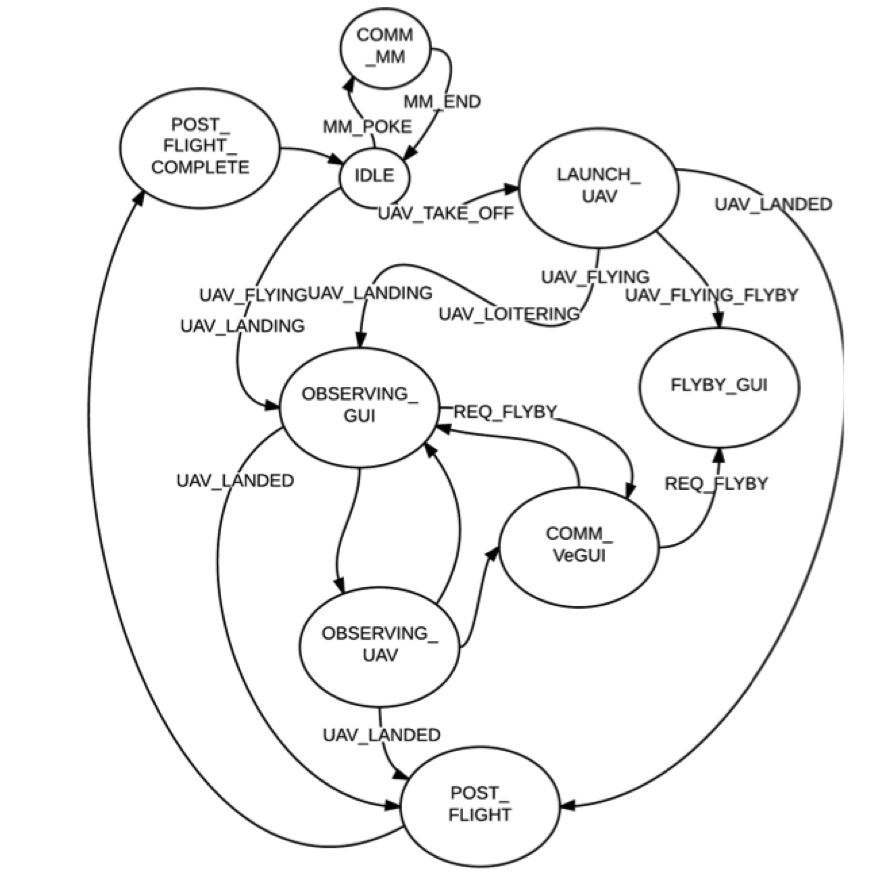
\includegraphics[height=2.4in]{DiRG.png}
\caption{Example actor model from prior work.}
\label{fig:dirg}
\end{figure}

We now present a formal description of each component of the model
\subsection{Actors}
Actors represent the human decision-makers and autonomous elements of the WiSAR team.  An actor is composed of a set of states $S$, an initial state $s_0$, a set of inputs from the environment $\Sigma_{\rm env}$, a set of inputs from other actors on the team $\Sigma_{\rm team}$, a set of outputs $\Lambda_{\rm out}$, a simple form of memory $\Omega_{\rm men}$, and a transition function that determines the next state from the inputs and memory $\delta$. Formally, we denote an actor as:
\begin{equation}
 	Actor = (S, s_0, \Sigma_{\rm env}, \Sigma_{\rm team}, \Lambda_{\rm out}, \Omega_{\rm mem},\delta)
 \label{eq:actor}
 \end{equation}
 
 \subsection{Outputs}
 An actor's output has two components: signals to other actors on a team and a {\em duration} parameter that represents the time required for the actor to complete its transition to the next state.  Thus, $\Lambda_{\rm out}=\Sigma_{\rm team} \times \Re^+$. The duration represents the relative difficulty of the
task(s) associated with the transition.  We justify this by assuming that
all tasks are performed at a constant rate, thus more difficult tasks take
longer, but note that future work should address this restrictive assumption.  
 
 \subsection{Transitions}
 
A transition is a relation on the cross product of inputs (a state, environment signal, signals from other actors, and element of memory)  with outputs (a next state, an output, and a modification to memory).  Thus,
\begin{equation}
 \delta:[S\times\Sigma_{\rm env}\times\Sigma_{\rm team}\times\Omega_{\rm mem}] \times [S\times \Sigma_{\rm team} \times \Omega_{\rm mem}], 
\end{equation} 
where we have used brackets to separate inputs from outputs.
 
Given an actor's current state, set of input signals, and memory, it is possible for multiple transitions to be possible.  This occurs because we assume that multiple environment signals or inter-actor signals may be occurring at the same time, which are all perceived by the actor since we assume perception is a parallel operation.  Thus, it is useful to explicitly note the number of possible transitions that are possible from a given state.   A transition is considered {\em enabled} when all of its input
requirements are met and {\em disabled} otherwise. 

\subsection{Current State}
When an actor is in a given state, it is useful to explicitly denote the set of enabled and disable transitions.  This allows a model-checker to use this information to create an estimate of algorithmic workload, where we assume that algorithmic workload is a function of the number of choices available to the actor.  Thus, we allow the current state to give an workload signal
 \begin{equation}
	s_0^{\rm work\  sig} = (T_{enabled}, T_{disabled}) : T_{enabled} \cap T_{disabled} = \emptyset
 \label{eq:state}
\end{equation}


\subsection{Declarative Memory }
Internal facts stored by an actor and used in decision making take the form of internal variables within an actor. A good example of this can be seen in the mission manager actor of our simulation. As the search begins, the mission manager receives a number of data items from the parent search, e.g. search area and target description. These items of information need to be communicated separately to different actors, so they must be stored internally in the mean time. 


\section{Directed Team Graph (DiTG)}

In order to measure human workload within the context of our model \cite{gledhill2013modelinguas} we
have defined the following set of core components which allows us to correlate
the activity within our model to human workload.  We call this framework the
directed team graph (DiTG).

\subsection{Conceptual Model}
In previous work we represented WiSAR as a collection of directed role graphs
(DiRGs)\cite{gledhill2013modelinguas}.  See figure~\ref{fig:ditg}.  As is common
when modeling human-automation interaction we have decided to model the DiRGs usings Mealy
state machines~\cite{bolton2013litreview}.  The DiTG formalizes this collection
by defining the communication mediums which unite the said DiRGs.  Using
multiple resource theory\cite{wickens2002multiple} as a guide we can explicitly
define the channels over which this communication occurs.  See
figure~\ref{fig:ditg_detail}.  The Actor state transitions then use these
channels to broadcast and receive inter-Actor communication.  

We hope to gain
insight into decreasing the system workload, and possibly combining roles, by
establishing metrics associated with the task model and model simulation.  These
metrics can then be used to determine if changes to the model represent a
decrease in operator workload.

\begin{figure}
\center
\setlength{\abovecaptionskip}{1mm}
\setlength{\belowcaptionskip}{1mm}
\setlength{\textfloatsep}{1mm}
\setlength{\floatsep}{1mm}
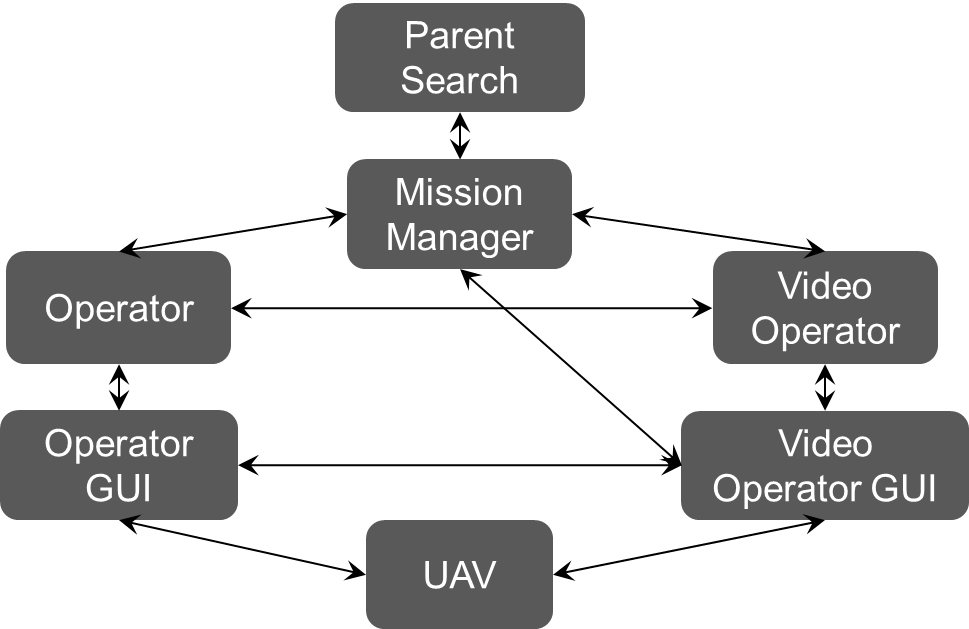
\includegraphics[height=2in]{ditg.png}
\caption{High Level DiTG}
\label{fig:ditg}
\end{figure}

\begin{figure}
\center
\setlength{\abovecaptionskip}{1mm}
\setlength{\belowcaptionskip}{1mm}
\setlength{\textfloatsep}{1mm}
\setlength{\floatsep}{1mm}
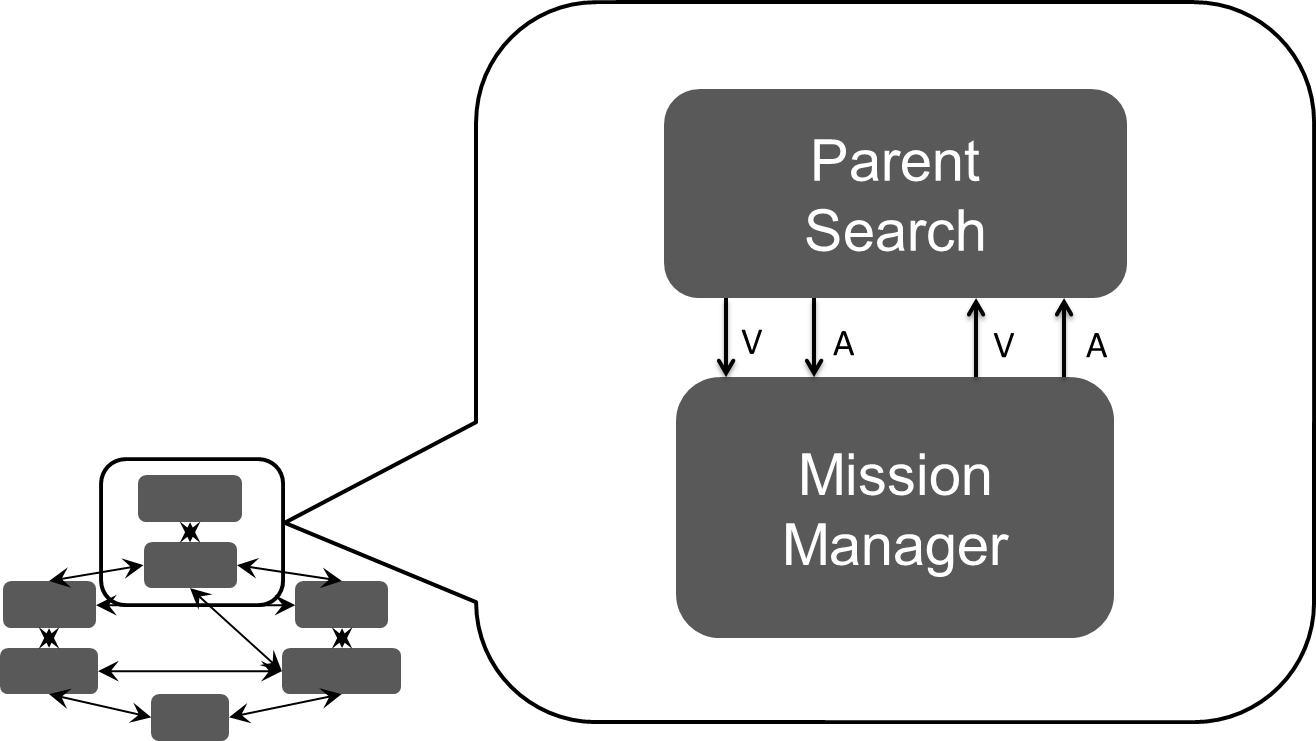
\includegraphics[height=1.9in]{ditg_detailed.png}
\caption{Detail view of DiTG: V is a Visual channel and A is an Audio channel}
\label{fig:ditg_detail}
\end{figure}

Formally, the models are the following mathematical structures:
 \begin{equation}
 	DiTG = (A, \Phi, \forall a_i \in A~ \exists \Phi_i \subset \Phi)
 \end{equation}

 \begin{equation}
 	Actor = (S, s_0, s_{current}, \Omega_A, \Sigma_A \subset \Phi, \Lambda_A
 	\subset \Phi)
 \label{eq:actor}
 \end{equation}

 \begin{equation}
	State = (T_{enabled}, T_{disabled})
 \label{eq:state}
\end{equation}

\begin{equation}
\begin{split}
	Transition = (\Omega_{input} \subset \Omega_A, \Sigma_{input} \subset \Sigma_A,\\
	\Omega_{value}^{input}, \Sigma_{value}^{input} \\
	\Omega_{output} \subset \Omega_A, \Lambda_{output} \subset \Lambda_A, \\
	\Omega_{value}^{output}, \Lambda_{value}^{output})
 \label{eq:transition}
 \end{split}
\end{equation}

\begin{equation}
\begin{split}
Channel (\phi) = (type \in (visual, audio), \\
value \in (null, *), 
 a_i^{source}, a_j^{target}) : i \neq j
 \label{eq:channel}
 \end{split}
\end{equation}

\begin{equation}
Declarative Memory(\omega) = value \in (null, *)
\end{equation}


where $A$ is a set of actors, $S$ a set of
states, $T$ a set of transitions, $\Phi$ a set of channels, $\Omega$ a set of
declarative memory, $\Sigma$ a set of input channels, and $\Lambda$ a set of
output channels.

\subsection{Framework Components}
\subsubsection{Actors}
Actors represent the agents within the system, while an Actor may be any type of agent for the context of workload we assume that an Actor is human.  An Actor is made up of a current state, the set of all possible states, declarative memory, and channels and are represented within the model as finite state machines.

\subsubsection{States}
States contain a set of all possible transitions to other Actor states.  While states typically represent the performance of a set of tasks they can also represent such things as emotion, fatigue, and neglect which is expressed in the transitions.  In this way an Actor�s current state represents its current decision making paradigm.

\subsubsection{Transitions}
A transition is composed of a set of required declarative memory and channel values, a set of declarative memory and channel output values, an end state, and a duration.  A transition is considered enabled when all of its input requirements are met.  The duration represents the relative difficulty of the task(s) associated with the transition.  We rationalize this by assuming that all tasks are performed at a constant rate, thus more difficult tasks take longer.

\subsubsection{Declarative Memory }
This memory represents internal facts stored by an Actor and used in decision making.  This memory takes the form of internal variables within an Actor, transitions can look for specific values on these variables to determine if they are enabled.

\subsubsection{Channels} 
Channels represent physical communication mediums that exist between Actors.  Each channel has a type (audio or visual), a buffer, a source, and a target.  The channel type is associated with the modality dimension of multiple resource theory while the source and target represent the stages dimension.  The source being the response and the target being perception/cognition.  We assume that all channels have a constant bandwidth, the longer a channel is in use the more data being sent across the channel.

\subsubsection{How it works}
We represent a system as a directed team graph (DiTG).  This is a collection of Actors connected to one another by a set of channels.  Whenever the state of the system changes an Actor will petition, from its current state, a list of enabled transitions thus defining what decisions can be made.  The Actor may then activate one of these transitions.  Transitions have two main states, active and fired.  When chosen a transition is made active, after the specified duration the transition fires.  When a transition becomes active it creates temporary output values for declarative memory and channels.  These temporary values are then applied to the actual declarative memory and channels when the transition fires.  

\subsection{Actor vs Tasks}
This architecture focuses on the Actor itself and less on the tasks performed by the Actor.  The difference being that Actor states can account for conditions on the Actor which affect performance and increase workload which cannot be seen simply by taking a set of tasks and examining their combined resource requirements.  For our model we never explicitly define a single task.  Instead we define Actors, States, and Transitions.  Each transition defines its own perceptual, cognitive, response, and declarative resources (Salvucci) which are not restricted to performing a single task.  The state contains all the possible transitions an Actor can choose from given its current state representing the performance of multiple tasks and procedural resources.  The Actor acts as the final cognitive resource by choosing which transition to follow.  In this way we achieve multi-tasking not by defining specific tasks but by defining the choices an Actor can make and the resources affected by each choice.

\section{Workload Metrics}
We are now in a position to combine the three categories of workload (cognitive, algorithmic, and temporal) with the formal model of the actors and team to generate a set of workload metrics.  Because the categories include many possible measurements that are beyond the scope of this paper, we use labels for the workload metrics that are slightly different from the workload categories.  As shown in Figure~\ref{fig:WorkloadMetrics}, cognitive workload or resource workload as it is termed in this work, is measured using metrics under the {\em resource} workload label, algorithmic under {\em decision}, and temporal workload is labeled the same. 


\begin{figure}[h]
\center
\setlength{\abovecaptionskip}{1mm}
\setlength{\belowcaptionskip}{1mm}
\setlength{\textfloatsep}{1mm}
\setlength{\floatsep}{1mm}
\scalebox{.8}{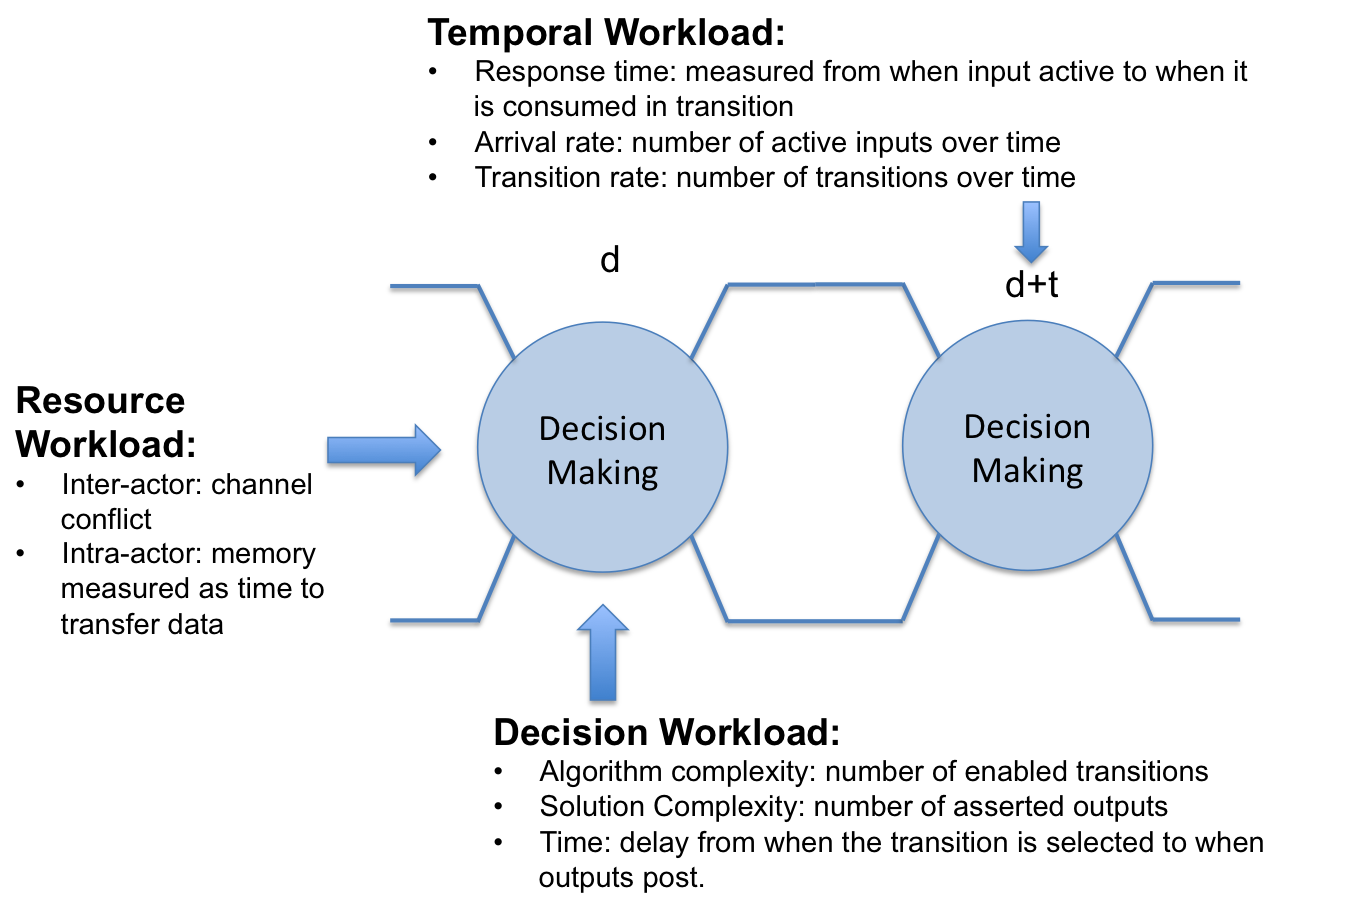
\includegraphics[height=2.5in]{WorkloadMetrics.png}}
\caption{Workload in the model.}
\label{fig:WorkloadMetrics}
\end{figure}

Resource workload is separated into both inter-actor communication and actor memory load. JPF listens to the output of the state transitions and records outputs to $\Omega_{\rm mem}$.  JPF also listens to all channel reads, noting how many communications are on the visual and auditory input channel, identified by the labeled edges of the DiTG, of each actor. 

Decision workload can be broken down into timing, complexity of the algorithm, and complexity of the solution. JPF is instrumented to measure timing as the time between when a transition becomes active and when it fires.  JPF is also instrumented to count the number of enabled transitions in each state as it is visited, giving us an $O(n)$ estimate of how the number of choices affects workload.   Finally, JPF is instrumented to count the number of output signals generated ($\Sigma_{\rm team}$), yielding an $O(n)$ estimate for the complexity of computing the required outputs of a state given its inputs.

Temporal workload includes three metrics: operations tempo, arrival rate, and response time.  JPF measures the average op-tempo counting how many transitions occur over a course of the simulation. JPF measures arrival rate by tracking the rate at which inputs become active. Finally, JPF measures response time by recording the time from when an input goes active to the point when it is read by the actor. \\


%\section{Predicting Workload}
	In the interest of consolidating operators it is critical to find an accurate measurement that detects situations that exceed the capacity of a given human. One way to detect this is by building a map of each actor's workload as a function of time. JPF is excellent in this regard as it explores all possible paths the model can take and returns the ones that violate the model's criteria. By augmenting our model with the metrics described above we can identify all possible areas of high workload. Once these critical sections have been identified we will either be able to minimize them by increasing the autonomy of the system or by rearranging task protocols to balance sections of high workload with other lower workload areas.

There are three techniques that we need to undergo in the validation process of our workload measurements. The first is consistency. As we analyze the maps produced in JPF we will need to verify that deviations in the workload are pridictable results. For example there should be no spikes in workload when all the actors are at rest. Once we've verified that the workload measurements are consistent with our understanding we will execute a sensitivity study. During this study we will instigate random permutations into the model and verify that the workload mutations correlate with those permutations. This study will verify that our understanding of the workload metrics implemented is accurate. Finally we will need to initiate a human study to verify that our metrics do in fact correlate with workload in humans. In this study we will use situations that caused spikes, low points, and high points of workload. By running our subjects through these same situations and receiving their feedback we will be able to verify that our metrics do in fact measure workload.
`\section{Results}
In the interest of consolidating operators it is critical to find an accurate measurement that detects situations that exceed the capacity of a given human. One way to detect this is by building a map of each actor's workload as a function of time. JPF explores all possible paths the model can take and returns the ones that violate the model's criteria. By augmenting our model with the metrics described above we can identify all possible areas of high workload. 

We propose three levels of increasing validity for evaluating the approach in the paper.  The first level, the one used in this paper, is to check for {\em consistency}.  We say that the approach is {\em consistent} if the workload peaks, valleys, and trends match what we know about a small set of given situations; in other words, the approach is consistent if it matches our expectations on tasks that we know a lot about.  

The second level, which is an area for future work, is to check for {\em sensitivity}.  We say that  the approach is sufficiently {\em sensitive} if we can use JPF to create new scenarios that have very high or very low workloads, and we can then generate a satisfactory explanation for the levels of workload by evaluating the new scenarios.  The third level, which is also an area of future work, is to {\em substantiate} workload levels using experiments with human participants by comparing the perceived workload of humans with those predicted by the model.

In this paper, we restrict attention to finding areas of high and low workload, and then checking these areas for consistency.  We evaluated consistency using two scenarios.  The first is when the Video Operator was able to identify the target during a flight without any complications occurring (see Figure~\ref{fig:WorkloadSim1}). For the first 40 time steps everything behaves as expected with low to moderate workload. An initial workload bump occurs as actors exchange information necessary to start a search.   At time step forty we see a dramatic deviation from the norm. This is a result of constant information passing between the GUIs and the operators. Since there is a constant passing of data between the machinery and the operators, it is only logical that the workload would increase substantially. However the results indicate that a weighting should be instigated to balance the three workload measures rather than allowing the single category to dominate the system. In our sensitivity study we will verify whether this is a fault in our metrics or if this one scenario lends itself to the distortion.  {\sc what happens to cause this spike, and why does it abate?}

\begin{figure}[h]
\center
\setlength{\abovecaptionskip}{1mm}
\setlength{\belowcaptionskip}{1mm}
\setlength{\textfloatsep}{1mm}
\setlength{\floatsep}{1mm}
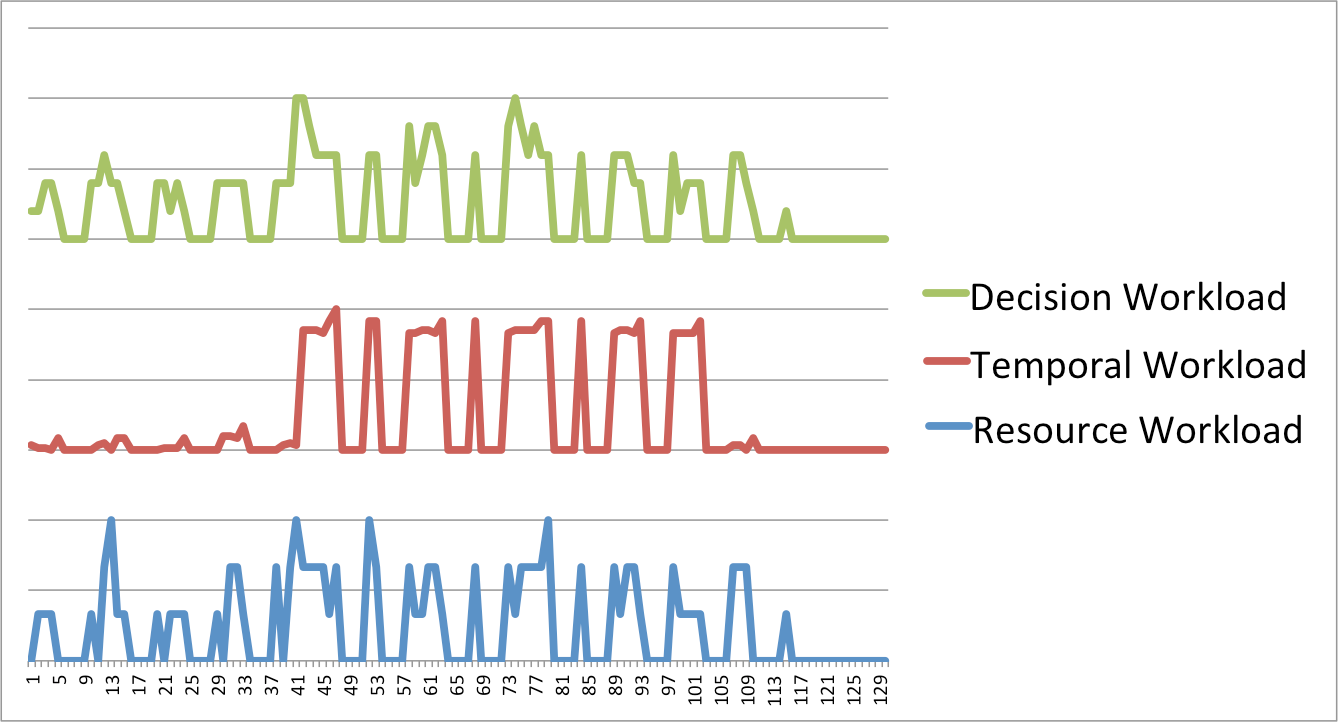
\includegraphics[height=2in]{WorkloadTargetSightingLabeled.png}
\caption{Workload over an uneventful flight.}
\label{fig:WorkloadSim1}
\end{figure}

The second simulation includes a situation where, after a short period of flight, the battery rapidly fails. In this particular situation the operator was unable to respond quickly enough to land the UAV before it crashed (see Figure~\ref{fig:WorkloadSim2}). There is an immediate spike in the temporal workload but, surprisingly,the workload then decreases back to normal levels in just five time steps. {\sc Why?} The second spike indicates an unexpected fluctuation in options among one of the actors, which will have to be investigated further to verify if this is an accurate response or if a flaw in the model had slipped past the verification stage of development. Finally, as would be expected, when the UAV crashed there was a small spike in the workload before everything came to a halt. 

\begin{figure}[h]
\center
\setlength{\abovecaptionskip}{1mm}
\setlength{\belowcaptionskip}{1mm}
\setlength{\textfloatsep}{1mm}
\setlength{\floatsep}{1mm}
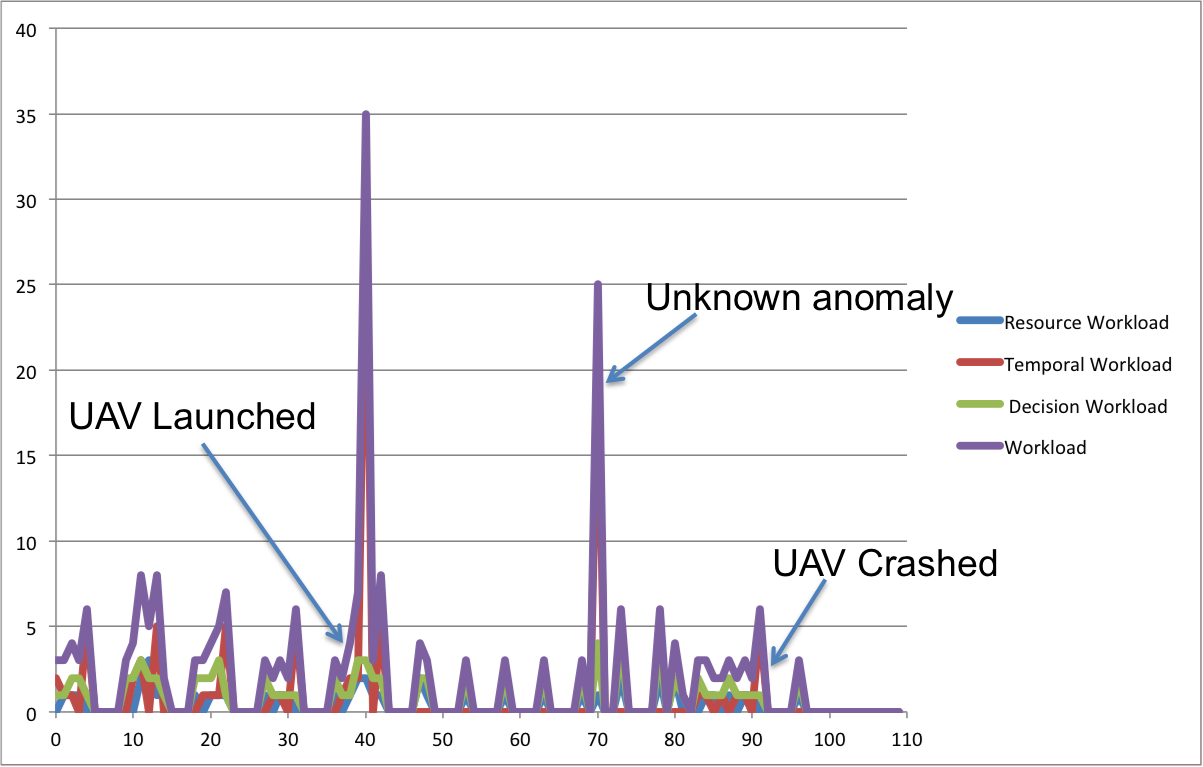
\includegraphics[height=2in]{WorkloadCrashedLabeled.png}
\caption{Emergency battery failure simulation}
\label{fig:WorkloadSim2}
\end{figure}

These two simulations demonstrate that workload rises and falls as expected and provide evidence that the approach is consistent with expectations.  However, there is also one event that was surprising and that needs further study.
\section{Related Work}

This work is an extension of previous work which focused on modeling human
machine systems, specifically WiSAR.  This work extends this model to
incorporate the measurement of workload~\cite{gledhill2013modelinguas}.

Multiple resource theory plays a key role in how we are measuring workload~\cite{wickens2002multiple}. The multiple resource model defines four categorical dimensions that
account for variations in human task performance.  A task can be represented as a vector of these dimensions.  Tasks interfere when they share resource dimensions.  Using these vectors, Wickens defined a basic workload measure consisting of the task difficulty (0,1,2) and the number of shared dimensions.  Using this metric it is possible to predict task interference by looking at tasks which use the same resource dimensions.  Our model differs in that we do not explicitly define tasks, instead we use Actor state transitions which may imply any number of concurrent tasks.  The transition then informs us of which resources are being used and for how long.  

Threaded cognition theory states that humans can perform
multiple concurrent tasks that do not require executive processes~\cite{salvucci2008threaded}.  By making a
broad list of resource assumptions about humans, threaded cognition is able to
detect the resource conflicts of multiple concurrent tasks.  Our model differs from
threaded cognition theory in that it does not allow learning nor does our model distinguish
between perceptual and motor resources. In almost all other aspects our model behaves in a similar fashion.

Related work on temporal workload has attempted to predict the number of UAVs an operator can
control, otherwise known as {\em fan-out}~\cite{cummings2007predicting,OlsenWood2004,CrandallEtAl2005}.  This work used queuing theory
to model how a human responds in a time sensitive multi-task environment.  Queuing theory is helpful in determining the temporal effects of task performance by measuring the difference between when a task was received and when it was executed.  Actors can only perform a single transition at a time, similar to queuing theory, but it is possible for each state to take input from multiple concurrent tasks which differs from standard models of queuing theory.

ACT-R is a cognitive architecture which attempts to model human cognition and
has been successful in human-computer interaction applications~\cite{anderson2004integrated,lebiere2013cognitive}.  The
framework for this architecture consists of modules, buffers, and a pattern-matcher which in many ways are very similar to our own framework.  The major
difference is that ACT-R includes higher levels of modeling detail, such as memory access
time, task learning, and motor vs perceptual resource differences.  Our model exists at a higher level of abstraction.

Complementary work has been done using Brahms.
%Brahms is a powerful language that allows for more detail than our research required.
Brahms is a powerful language that allows for far more detail than we found our research required.
In addition at the time we started developing our model Brahms lacked some of the tools we needed for extracting workload data from the model. Because of this we found that Java in conjunction with JPF made a better match for our needs.

\section{Conclusion and Future Work}
This paper has analyzed the role workload analysis plays in the optomization process of a semiautomated system. Results have shown that an effective modeling system can be based off of Moore finite state machines connected together via a DiTG. Preliminary analysis of the model revealed that communication is a primary cause of spikes in workload. This concept is benificial since data transfer can be executed effectively using automation allowing us to smooth out the peaks in our simulations.

Since optimal workload metrics are desired, we are proceeding with further
automation of metric analysis. While we may find a cumulatively middle path, it may be interspersed with workload peeks and valleys. These are like miniature instances of high and low workload, and they cause the same problems we are trying to avoid. Java Pathfinder (JPF) has been an exceptional tool in finding all the paths that the system can take. Since it produces nearly a million lines of data, finding paths with a stable workload must be automated.

For our next steps we have several basic plans. We will also be adding an actor to handle sense and avoidance operations. In addition to that it is necesarry to implement a way to evaluate the cost of errors in decision making. There will be certain tasks that cannot be automated because the cost of failure requires a human's undivided attention. First we will be undergoing a sensitivity study, followed by a field test. One we've verified that our system analyzes workload correctly We will branch our research into two separate directions. The first area will consist of generated an optimized GUI for the WiSAR system, hopefully to allow a single operator to take full control of the WiSAR system. While the second branch will be formulated a generalized model that will have application across the board for UAV systems.



% use section* for acknowledgement
% use section* for acknowledgement
\section*{Acknowledgment}
% optional entry into table of contents (if used)
% \addcontentsline{toc}{section}{Acknowledgment}
The authors would like to thank the NSF IUCRC Center for Unmanned Aerial Systems, and the participating industries and labs, for funding the work.


% can use a bibliography generated by BibTeX as a .bbl file
% standard IEEE bibliography style from:
% http://www.ctan.org/tex-archive/macros/latex/contrib/supported/IEEEtran/bibtex
\bibliographystyle{aaai}
% argument is your BibTeX string definitions and bibliography database(s)
\bibliography{references,standard3}


% that's all folks
\end{document} 